\documentclass[10pt,landscape]{article}
\usepackage{amssymb,amsmath,amsthm,amsfonts}
\usepackage{multicol,multirow}
\usepackage{calc}
\usepackage{ifthen}
\usepackage{graphicx}
\usepackage{xcolor}
\usepackage{cprotect}
\usepackage[utf8]{inputenc}
\usepackage{enumitem}
\usepackage{listings}
\usepackage[landscape]{geometry}
\usepackage[colorlinks=true,citecolor=blue,linkcolor=blue]{hyperref}
\usepackage{fancyhdr}

\lstset{
    tabsize=2,    
%   rulecolor=,
    language={SQL},
        captionpos = t,
        basicstyle = \scriptsize\ttfamily,
        frame=lines,
        numbersep=4pt,
        numbers=left,
        numberstyle=\tiny,
        backgroundcolor=\color{white},
        columns=fixed,
        extendedchars=false,
        breaklines=true,
        prebreak = \raisebox{0ex}[0ex][0ex]{\ensuremath{\hookleftarrow}},
        frame=single,
        showtabs=false,
        showspaces=false,
        showstringspaces=false,
        keywordstyle=\color[rgb]{0,0,1},
        keywordstyle=[2]\color{gray},
        commentstyle=\color{teal},
        stringstyle=\color{red},
        numberstyle=\color[rgb]{0.205, 0.142, 0.73},
        framesep=0pt
}

\newenvironment{tightcenter}{%
  \setlength\topsep{0pt}
  \setlength\parskip{0pt}
  \begin{center}
}{%
  \end{center}
}

\def\ojoin{\setbox0=\hbox{$\bowtie$}%
  \rule[-.02ex]{.25em}{.4pt}\llap{\rule[\ht0]{.25em}{.4pt}}}
\def\leftouterjoin{\mathbin{\ojoin\mkern-5.8mu\bowtie}}
\def\rightouterjoin{\mathbin{\bowtie\mkern-5.8mu\ojoin}}
\def\fullouterjoin{\mathbin{\ojoin\mkern-5.8mu\bowtie\mkern-5.8mu\ojoin}}

\ifthenelse{\lengthtest { \paperwidth = 11in}}
    { \geometry{top=.25in,left=.25in,right=.25in,bottom=.25in} }
	{\ifthenelse{ \lengthtest{ \paperwidth = 297mm}}
		{\geometry{top=1cm,left=1cm,right=1cm,bottom=1cm} }
		{\geometry{top=1cm,left=1cm,right=1cm,bottom=1cm} }
	}
\pagestyle{empty}
\makeatletter
\renewcommand{\section}{\@startsection{section}{1}{0mm}%
                                {-1ex plus -.5ex minus -.2ex}%
                                {0.5ex plus .2ex}%x
                                {\normalfont\large\bfseries}}
\renewcommand{\subsection}{\@startsection{subsection}{2}{0mm}%
                                {-1explus -.5ex minus -.2ex}%
                                {0.5ex plus .2ex}%
                                {\normalfont\normalsize\bfseries}}
\renewcommand{\subsubsection}{\@startsection{subsubsection}{3}{0mm}%
                                {-1ex plus -.5ex minus -.2ex}%
                                {1ex plus .2ex}%
                                {\normalfont\small\bfseries}}
\makeatother
\setcounter{secnumdepth}{0}
\setlength{\parindent}{0pt}
\setlength{\parskip}{0pt plus 0.5ex}

\title{CS2102-cheatsheet}
% -----------------------------------------------------------------------

\begin{document}

\raggedright
\footnotesize


\begin{multicols*}{3}
    \begin{tiny}
        \small{\textbf{CS2102 Cheatsheet AY22/23 S2 || \href{https://github.com/JasonYapzx}{@JasonYapzx}}} \\
   \end{tiny}
\setlength{\premulticols}{0.5pt}
\setlength{\postmulticols}{0.5pt}
\setlength{\multicolsep}{0.5pt}
\setlength{\columnsep}{0.5pt}

\begin{itemize}[topsep=0pt,noitemsep,wide=0pt, leftmargin=\dimexpr\labelwidth + 2\labelsep\relax]
    \item \underbar{A}tomiticty - all/none of T reflected in the database
    \item \underbar{C}onsistency - T guarantees the correct state 
    \item \underbar{I}solation - T isolated from effects of concurrent transactions
    \item \underbar{D}urability - after T, effects are permanent
    \item \textit{Data model:} collection of concepts for describing data.
    \item \textit{Schema:} desc. of structure of a database using a data model.
    \item \textbf{superkey}: subset of attributes that \underline{uniquely identifies} a tuple
    \item \textbf{key}: is a \textbf{\textit{superkey}} that is also \underline{minimal} $\rightarrow$\ no proper subset of the key is a superkey. (cannot be made smaller) $\neq$ smallest
    \item \textbf{candidate keys}: set of \underline{all \textbf{keys}} of a given relation
    \item \textbf{primary key}: \underline{selected \textbf{candidate keys}}, and they CANNOT be NULL. To simplify our notation, we \underline{underline} our primary keys in the schema notation.
    \item \textbf{Foreign Keys:} subset of attributes of relation \textit{R$_1$} that \underline{refers to the \textbf{PK}} of relation \textit{R$_2$}.
    \footnotesize {$\rightarrow$\ \textit{R$_1$}: referencing, \textit{R$_2$}: referenced relation}
    \item \textbf{Requirements}: each FK in \textit{R$_1$} must appear as a PK in \textit{R$_2$} \underline{\textbf{OR}} be NULL value (in a tuple, contain at least 1 NULL value)
\end{itemize}

\textbf{\underline{Data Types in SQL}}
\textbf{boolean:} \verb|true/false| (\verb|null| == unknown) | \textbf{integer:} signed 4 byte integer
| \textbf{float8:} double-precision floating point number (8 bytes) | \textbf{numeric:} arbitrary precision floating point number 
| \textbf{numeric(p, s):} max total of $p$ digits with max of $s$ decimals | \textbf{char(n):} fixed-length string consisting of n characters
| \textbf{varchar(n):} variable-length string up to n characters | \textbf{text:} variable-length character string
| \textbf{date:} calender date (year, month, day) | \textbf{timestamp:} date and time 

\textbf{Is Null Predicate}: \verb|x IS NULL|

\textbf{Is Distinct from Predicate:} \verb|x IS DISTINCT FROM y|

\textbf{non-null:} \verb|name     varchar(100) NOT NULL,|

\textbf{unique:} \verb|studentId     INT UNIQUE,| or
\verb|unique (city, state) -- at bottom|

\textbf{primary key:}
\verb|studentId   INT PRIMARY KEY|
or \verb|PRIMARY KEY (eid, pname), -- at bottom|

\textbf{foreign key:} \verb|studentId     INT REFERENCES Student (id)|
or \verb|FOREIGN KEY (a, b) REFERENCES Other (a, b) -- at bottom|

\textbf{\underline{Foreign Key Constraints Violations}} \\ 
\textit{No Action:} Rejects action if violates constraint (default) | \textit{Restrict:} Same as No action but constraint checking is not deffered
| \textit{Cascade:} Propagates delete/update to referencing tuples | \textit{Set NULL:} Updates foreign keys to NULL
| \textit{Set Default:} Updates foreign keys to some value, need to speicfy this value as the referecing column 
and must meet foreign key constraints otherwise fails


\textbf{\underline{CREATE/ALTER/DROP Table}}
\begin{lstlisting}
ALTER TABLE <table_name> [ALTER / ADD / DROP] 
    [COLUMN / CONSTRAINT] <name> <changes>;
DROP TABLE [IF EXISTS] // no error if does not exist
<table_name>[, <table_name> [, <table_name> [...]]] 
    [CASCADE]; // also delete referencing table
\end{lstlisting}

% \textbf{Defferable Constraints:}
% \textit{unique}, \textit{PK} and \textit{FK} constraints
% \begin{itemize}[topsep=0pt,noitemsep,wide=0pt, leftmargin=\dimexpr\labelwidth + 2\labelsep\relax]
%     \item \verb|DEFERRABLE INITIALLY DEFFERED|: at the end of transaction.
%     \item \verb|DEFERRABLE INITIALLY IMMEDIATE|: after each statement.
%     \item \verb|NOT DEFFERABLE|: default for constraints
% \end{itemize}

\textbf{\underline{Entity-Relationship (ER) Model}}
\begin{scriptsize}
    \textit{Entity}: Real-world object distinguishable from other objects \\
    \textit{Attribute}: Specific information describing an entity, ovals \\
    \textit{Entity set}: Collection of similar entities, rectangles \\
    \textit{Key}: Represented as underlined attributes \\
    \textit{Relationship}: Association among 2 or more entries
    \textit{Relationship set}: Collection of similar relationships, represented by diamonds. Attributes used to describe information about relationships.
\end{scriptsize}

\textbf{\underline{Relationship Constraints}}
\begin{multicols*}{2}
    \begin{itemize}[topsep=0pt,noitemsep,wide=0pt, leftmargin=\dimexpr\labelwidth + 2\labelsep\relax]
        \item \textit{Key Constraint}: $E$ \textbf{at most one} of $R$ ($\rightarrow$)
        \item \textit{Total Part Constraint}: $E$ \textbf{at least 1} of $R$ ($=$)
        \item \textit{Key \& Total Part Constraint}: $E$ \textbf{exactly 1} of $R$ ($\Rightarrow$)\\
        \item \textit{Weak Entity Set}: $E$'s identifying owner is $EE$, identifying relationship set: $R$. $E$ does not have own key to be uniquely indentified.
        \item \textit{Partial Key}: Set of attributes of a weak entity set that uniquely identifies a weak entity for a given owner entity.
    \end{itemize}
\end{multicols*}
\begin{enumerate}[topsep=0pt,noitemsep,wide=0pt, leftmargin=\dimexpr\labelwidth + 2\labelsep\relax]
    \item Can \textbf{PK} be used to \underline{uniquely identify} other attributes
    \item Is the LOWER BOUND satisfied in the schema?
    \item Is the UPPER BOUND satisfied in the schema?
\end{enumerate}

\textbf{Extended Notations - Aggregation}
\begin{multicols*}{2}
    Abstraction that treats relationships as \underline{higher-level} entities.
    Treat it as a relation class in OOP.
\includegraphics*[scale=0.25]{images/aggregation.jpg}
\end{multicols*}
\begin{multicols*}{2}
\textbf{ISA:} Every entity subclass is an entity in its superclass.
\framebox{\parbox{\dimexpr\linewidth-2\fboxsep-2\fboxrule}{%
\textbf{Overlap:} Can a superclass belong to \underline{multiple} subclasses? \\
\textbf{Covering:} Must a superclass belong to \underline{at least one} subclass?}} 
\includegraphics*[width=2.5cm]{images/isaconstraints.jpg}
\end{multicols*}

\textbf{\underline{Subqueries}}
\begin{itemize}[topsep=0pt,noitemsep,wide=0pt, leftmargin=\dimexpr\labelwidth + 2\labelsep\relax]
    \item WHERE - Pattern Matching: \verb|_| matches \underline{any} single character, \verb|%| matches any sequence of \underline{0 or more} characters.
    \begin{itemize}[topsep=0pt,noitemsep,wide=0pt, leftmargin=\dimexpr\labelwidth + 2\labelsep\relax]
        \item start w/ `Ma', end with `a': \verb|WHERE pizza LIKE 'Ma%a'|
        \item starts w/ ‘A’ and $\geq$ 5 chars: \verb|WHERE name LIKE 'A____%'|
    \end{itemize}
    \item SET OPERATIONS \verb|Q1 UNION/INTERSECT/EXCEPT [ALL] Q2| \verb|ALL| does not remove duplicates
    \item JOIN OPERATIONS: Most common in practice: \underline{cross product} + \underline{selection condition} + \underline{attribute selection}
\end{itemize}

\textbf{Scalar Subqueries:} A query that returns at \underline{most a single value}.
\textbf{[ NOT ] IN:} returns exactly one column. \\ 
    $\bullet$ \verb|IN| returns \verb|TRUE| if \verb|<expr>| matches \underline{any} subquery row \\ 
    $\bullet$ \verb|NOT IN| returns \verb|TRUE| if \verb|<expr>| matches \underline{no} subquery row
\textbf{ANY/SOME:} Expression \verb|<expr>| is compared
to each row from subquery using the operator \verb|<op>|, returns \verb|TRUE| if comparison evaluates to \verb|TRUE| for \textbf{at least one row} in the subquery \\ 
\textbf{ALL:} same as \verb|ANY| except needs \textbf{ALL} rows \\ 
\textbf{[ NOT ] EXISTS:} May return any number of columns \\ 
    $\bullet$ \verb|EXISTS| returns \verb|TRUE| if the subquery returns \underline{at least one row} \\ 
    $\bullet$ \verb|NOT EXISTS| returns \verb|TRUE| if the subquery returns no row

\framebox{\parbox{\dimexpr\linewidth-2\fboxsep-2\fboxrule}{% 
$\star$ Not all constructs required: IN $\equiv$ ANY $\equiv$ EXIST
}} \newline

\textbf{Order By:} \verb|ORDER BY <attribute> ASC/DESC|: (default for SQL, ASC can be removed).
If duplicate removal needed, attribute being sorted \textbf{must} appear in \verb|SELECT|. Sorting w.r.t multiple attributes /  differing order supported

\textbf{LIMIT k:} Return the \underline{first*} \verb|k| rows of the result table \\ 
\textbf{OFFSET i:} Specify the position of the \underline{first} row to be considered
$\star$ \verb|LIMIT| and \verb|OFFSET| typically meaningful only in with \verb|ORDER BY|

\textbf{\underline{Aggregate Functions}}
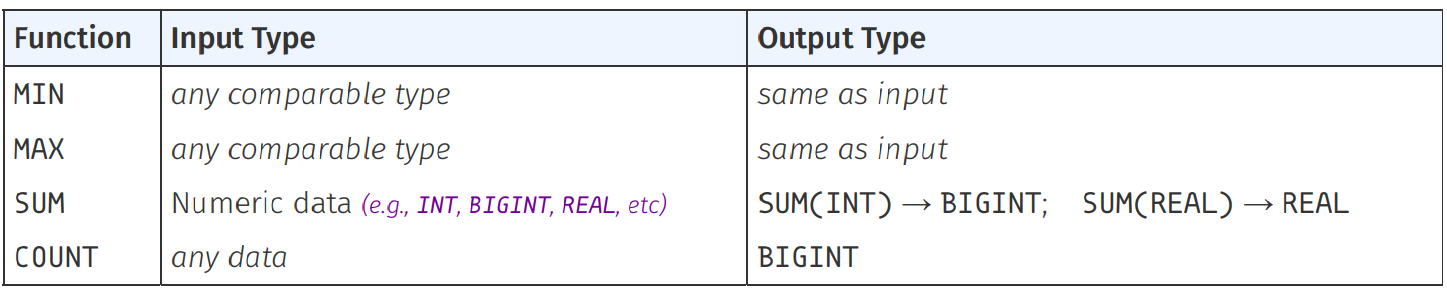
\includegraphics[height=1.3cm, width=8.5cm]{images/aggregatefunction.png}
Aggregate functions compute a \textbf{\textit{single value}} from a set of tuples.

If \verb|R| is empty set with \verb|B| attribtue, \verb|COUNT(*) = 0, COUNT(B) = 0|, \verb|SELECT aggrFn(B) FROM R = NULL|. 
If \verb|S| is non-empty relation with $n$-rows of attribute \verb|A| with only \verb|NULL| values in table
\verb|COUNT(*) = n, COUNT(A) = 0| and \verb|SELECT aggrFn(A) = NULL|

\textbf{\underline{Grouping (GROUP BY):}} 
\framebox{\parbox{\dimexpr\linewidth-2\fboxsep-2\fboxrule}{%
$\star$ f column A$_i$ appears in SELECT, one condition must hold
\begin{itemize}[topsep=0pt,noitemsep,wide=0pt, leftmargin=\dimexpr\labelwidth + 2\labelsep\relax]
    \item A$_i$ appears in the GROUP BY clause
    \item A$_i$ appears as input of aggregation function in SELECT clause
    \item The pkey of R appears in the GROUP BY clause
\end{itemize}
}}   

\textbf{\underline{HAVING:}} \verb|WHERE| clauses only works on each row. If we were to use \verb|WHERE p < AVG(p)|, any p that does not fit this condition
will be removed, resulting in \verb|AVG(p)| to change. \verb|HAVING| instead aggregates the condition for each group defined by \verb|GROUP BY|.
\framebox{\parbox{\dimexpr\linewidth-2\fboxsep-2\fboxrule}{%
$\star$ If column A$_i$ appears in HAVING, one condition must hold
\begin{itemize}[topsep=0pt,noitemsep,wide=0pt, leftmargin=\dimexpr\labelwidth + 2\labelsep\relax]
    \item A$_i$ appears in the GROUP BY clause
    \item A$_i$ appears as input of aggregation function in HAVING clause
    \item The pkey of R appears in the GROUP BY clause
\end{itemize}
}}   

\textbf{\underline{Conceptual Evaulation of Queries}}
1. \verb|FROM|: Compute cross-product of all tables in \verb|FROM|.
2. \verb|WHERE|: Filter (keep) tuples evaulate to \verb|TRUE| on \verb|WHERE|.
3. \verb|GROUP BY|: Partition tables into groups wrt to grouping attributes.
4. \verb|HAVING|: Filter groups evaulate to \verb|TRUE| on \verb|HAVING|.
5. \verb|SELECT|: Remove all attributes not specified in \verb|SELECT| (remove dup if \verb|DISTINCT|).
6. \verb|ORDER BY|: Sort tables based on specified attribute.
7. \verb|LIMIT/OFFSET|: Filter tuples based on their order in the table.

\cprotect\textbf{Conditional Expressions: \verb|CASE|}
Only one of the results will be returned, \verb|ELSE| optional, \verb|NULL| returned if no condition matched.
\verb|CASE WHEN <condition_1> THEN <result_1> ... ELSE result_0 END|


\cprotect\textbf{\verb|COALESCE|}
Returns first non-NULL value in list of input arguments (order of \verb|order| matters!) \verb|COALESCE(<value_1>, <value_2>, <value_3>, ...)|

\cprotect\textbf{\verb|NULLIF|}
Returns NULL if \verb|<value_1>| = \verb|<value_2>|, else \verb|<value_1>|

\begin{multicols*}{2}
\textbf{\underline{Common Table Expression}}
\begin{lstlisting}
WITH
CTE_1 AS ( Q_1 ),
...
CTE_n AS ( Q_n )
Q_0 -- main SELECT statement:
\end{lstlisting}
\begin{itemize}[topsep=0pt,noitemsep,wide=0pt, leftmargin=\dimexpr\labelwidth + 2\labelsep\relax]
    \item Each CTE$_i$ can reference any other CTE$_j$ that has been declared before (i.e., j $<$ i)
    \item Main SELECT statement Q$_0$ can reference any possible subset of all CTE$_i$
    $\rightarrow$ Any CTE$_i$ not referenced can be deleted 
\end{itemize}
\end{multicols*}

\textbf{\underline{Views}}
Usually need parts of the table, restrict access to table for certain users,
and often use the same queries and subqueries frequently. \verb|CREATE OR REPLACE VIEW <name> AS <query>|

\textbf{\underline{Functions}}
\begin{lstlisting}
CREATE OR REPLACE FUNCTION 
    markCnt(OUT TopMark INT, OUT Cnt INT)
RETURNS SETOF RECORD Scores AS $$
    SELECT Mark, COUNT(*) FROM Scores GROUP BY Mark;
$$ LANGUAGES sql;
\end{lstlisting}
\verb|SETOF| used when want to return \underline{multiple} records.
\verb|RECORDS| used for only \underline{1} record, and not in the current schema.
\verb|SETOF RECORDS| is used for multiple tuples, not in the current schema.
\verb|TABLE| is similar to \verb|SETOF RECORDS|.

\textbf{\underline{Procedures}}
No return value/tuple needed, may use \textbf{SQL procedures}. \verb|CALL transfer('Alice', 'Bob', 100);|
\verb|CREATE OR REPLACE PROCEDURE g(x int) as $$|

\begin{multicols*}{2}
\textbf{\underline{Recursive Queries}}
\begin{lstlisting}
WITH RECURSIVE
    CTE_name AS (
        Q_1
        UNION [ ALL ]
        Q_2 ( CTE_name )
    )
Q_0 ( CTE_name )
\end{lstlisting}
\begin{itemize}[topsep=0pt,noitemsep,wide=0pt, leftmargin=\dimexpr\labelwidth + 2\labelsep\relax]
    \item Q$_1$ is non-recursive
    \item Q$_2$ is recursive and can reference CTE$_{name}$
    \item Query is evaluated `lazily', stops when a fixxed-point is reached
\end{itemize} \break
\begin{lstlisting}
WITH RECURSIVE
Linker(to_stn, stops) AS (
    SELECT to_stn, 0
    FROM MRT
    WHERE fr_stn = 'NS1'
    UNION ALL
    SELECT M.to_stn, L.stops + 1
    FROM Linker L, MRT M
    WHERE L.to_stn = M.fr_stn
        AND L.stops < 2
)
SELECT DISTINCT (to_stn)
FROM Linker;
\end{lstlisting}
\end{multicols*}

\textbf{\underline{Variables and Control Structures}}
\begin{lstlisting}
AS $$ DECLARE             |   IF condition1 THEN
    temp_val INTEGER;     |      statement1;
BEGIN -- functinon body   |   ELSEIF condition2 then
END;                      |      statement2;
$$ language plpgsql;      |   ELSE
__________________________|      else-statement;
LOOP                      |   END IF;
    EXIT WHEN condition;  |
    -- loop body;         |
END LOOP;                 |
\end{lstlisting}
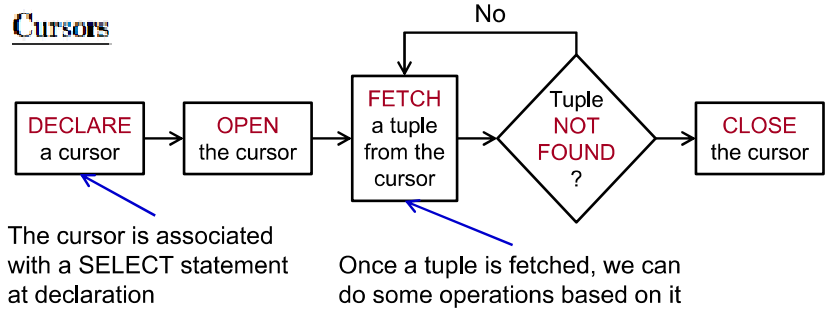
\includegraphics[width=6.5cm, height=1.8cm]{images/cursorworkflow.png}
\begin{lstlisting}
CREATE OR REPLACE FUNCTION score_gap()
RETURNS TABLE(name TEXT, mark INT, gap INT) AS $$
DECLARE // Declares cursor variable
    curs CURSOR FOR (SELECT * FROM Scores ORDER BY Mark DESC);
    r RECORD;
    prv_mark INT;
BEGIN
    prv_mark := -1;
    OPEN curs;   
    LOOP     
        FETCH curs INTO r; EXIT WHEN NOT FOUND; 
        name := r.Name; mark := r.Mark;
        IF prv_mark >= 0 THEN gap := prv_mark - mark;
        ELSE gap := NULL; END IF;
        RETURN NEXT; prv_mark := r.Mark;   
    END LOOP;
    CLOSE curs;               
END;
$$ LANGUAGE plpgsql;
\end{lstlisting}
$\bullet$ \verb|FETCH PRIOR/FIRST/LAST FROM cur INTO r| $\rightarrow$ fetch the prior/first/last row \\
$\bullet$ \verb|FETCH ABSOLUTE 3 FROM cur INTO r| $\rightarrow$ fetch the 3$^{rd}$ tuple

\textbf{\underline{Triggers $\leftrightarrow$ Trigger Functions}}

\begin{lstlisting}
CREATE TRIGGER trigger AFTER INSERT ON Table
FOR EACH ROW EXECUTE FUNCTION trigger_fn();
CREATE OR REPLACE FUNCTION trigger_fn() 
RETURNS TRIGGER AS $$
BEGIN /*Trigger Logic*/  END; $$ LANGUAGE plpgsql;
\end{lstlisting}
$\bullet$ \verb|RETURNS TRIGGER|' indicates that this is a trigger function, only \verb|RETURNS TRIGGER| allowed as only \verb|TRIGGER| has access to the \verb|NEW|. \\
$\bullet$ \verb|NEW| refers to new row inserted into Scores \\
$\bullet$ \verb|CURRENT_DATE| returns the current date \\ 
$\bullet$ \verb|TG_OP|: operation that activates trigger: \verb|INSERT|, \verb|UPDATE|, \verb|DELETE| \\
$\bullet$ \verb|TG_TABLE_NAME|: name of table that cause trigger invocation \\
$\bullet$ \verb|OLD|: old tuple being updated/deleted 

\textbf{\underline{Return Values of Trigger Function}}
\begin{itemize}[topsep=0pt,noitemsep,wide=0pt, leftmargin=\dimexpr\labelwidth + 2\labelsep\relax]
    \item \verb|BEFORE INSERT|: non-null \verb|t| | \verb|t| inserted, null \verb|t| | no insertion
    \item \verb|BEFORE UPDATE|: non-null \verb|t| | \verb|t| updated, null \verb|t| | no update
    \item \verb|BEFORE DELETE|: non-null \verb|t| | \verb|t| deleted, null \verb|t| | no deletion
    \item \verb|AFTER INSERT/UPDATE/DELETE| return value does not matter
    \item \verb|INSTEAD OF| non-null \verb|t| | proceed, null \verb|t| | ignore operations on current row. If a \verb|BEFORE|
    row-level trigger returns \verb|NULL|, then all subsequent triggers on same row are omitted. (\verb|VIEW|s only)
\end{itemize}

\cprotect\textbf{Trigger Levels | \verb|FOR EACH|}
\verb|ROW|: \textbf{row-level} trigger that executes trigger function for every tuple encountered. \\
\verb|STATEMENT|: \textbf{statement-level} trigger that executes the trigger function \underline{only once}.
\cprotect\textbf{\verb|EXCEPTION|s} raised to ignore operations for statement-level triggers. \verb|NOTICE|s does not stop operations \\ 
\textbf{\underline{Trigger Condition}} Has the following rules: e.g. \verb|FOR EACH ROW WHEN (NEW.Name = 'Hello') EXECUTE|
\begin{multicols*}{2}
    \begin{itemize}[topsep=0pt,noitemsep,wide=0pt, leftmargin=\dimexpr\labelwidth + 2\labelsep\relax]
        \item No \verb|SELECT| in \verb|WHEN()|
        \item No \verb|OLD| in \verb|WHEN()| for \verb|INSERT|
        \item No \verb|NEW| in \verb|WHEN()| for \verb|DELETE|
        \item No \verb|WHEN| for \verb|INSTEAD OF|
    \end{itemize}
\end{multicols*}

\textbf{\underline{Deffered Triggers}}
\begin{lstlisting}
CREATE CONSTRAINT TRIGGER bal_check_trigger
AFTER INSERT OR UPDATE OR DELETE ON Account
DEFFERABLE INITIALLY DEFERRED
FOR EACH ROW EXECUTE FUNCTION bal_check_func();
\end{lstlisting}
$\bullet$ \verb|CONSTRAINT| + \verb|DEFERRABLE|: trigger can be deffered \\
$\bullet$ \verb|INITIALLY DEFFERED|: by default, trigger is deffered. \verb|INITIALLY IMMEDIATE| trigger not deffered by default. \\
$\bullet$ DEFFERED Triggers only work for \verb|AFTER| and \verb|FOR EACH ROW|, \verb|AFTER| so that it can be executed after main operation.



\begin{itemize}[topsep=0pt,noitemsep,wide=0pt, leftmargin=\dimexpr\labelwidth + 2\labelsep\relax]
    \item Order of trigger activation:
     \verb|BEFORE| statement-level triggers $\rightarrow$ \verb|BEFORE| row-level triggers
     $\rightarrow$ \verb|AFTER| row-level triggers  \verb|AFTER| statement-level triggers
    \item Within each category, triggers activated in alphabetic order
\end{itemize}

\textbf{\underline{Functional Dependencies}:} $A$ $\rightarrow$ $B$ means $A$ decides $B$, if 2 rows have same $A$, then they have same $B$ also. \\
\textbf{Armstrong's Axioms}
\begin{enumerate}[topsep=0pt,noitemsep,wide=0pt, leftmargin=\dimexpr\labelwidth + 2\labelsep\relax]
    \begin{multicols*}{2}
    \item \textbf{Reflexivity:} AB $\rightarrow$ A
    \item \textbf{Augmentation:} If A $\rightarrow$ B, then AC $\rightarrow$ BC
    \item \textbf{Transitivity:} If A $\rightarrow$ B, and B $\rightarrow$ C then A $\rightarrow$ C
    \item \textbf{Decomposition:} If A $\rightarrow$ BC then A$\rightarrow$ B and A $\rightarrow$ C
    \item \textbf{Union:} If A $\rightarrow$ B and A $\rightarrow$ C then A $\rightarrow$ BC
    \end{multicols*}
\end{enumerate}

\textbf{\underline{Closure:}}
Four attributes \textit{A, B, C, D}. Given that B $\rightarrow$ D, DB $\rightarrow$ A, AD $\rightarrow$ C, check if B $\rightarrow$ C holds.
\{ B \}$^+$ = \{ B \} = \{ B, D \}, since B $\rightarrow$ D
= \{ B, D, A \}, since DB $\rightarrow$ A = \{ B, D, A, C \}, since AD $\rightarrow$ C. \{ B, D, A, C \} reffered to as \textit{closure} of B, which is the set of componenets that can be `activated' by B

\textbf{Superkeys:} set of attributes that decides all other attributes. \\ 
\textbf{Keys:} Superkey that is minimal. Whether or not a table has \textit{redundancy} or \textit{anomalies} depend on keys. \textbf{Prime Attribute:}
Attribute that appears in a key.
\textbf{Finding Keys:} any attribute that \textit{does not appear in RHS}, it \textbf{must be in every key}. 
If key: e.g. \{ A, C \} able to activate all other attributes, do no need to check supersets for \textit{keys} as keys are \underline{minimal}

\textbf{\underline{Normal Forms}}
BCNF requires that if there is any \textbf{non-trivial} and \textbf{decomposed} FD A$_1$A$_2$...A$_n$ $\rightarrow$ B, then A$_1$A$_2$...A$_n$ must be a superkey.
More simply, BCNF requires LHS to be super keys, prevent redundancy. \\ 
\textbf{Decomposed FD:} FD whose RHS only has 1 attribute  
\textbf{Non-Trivial:} FD whose RHS does not appear in LHS 
\textbf{Completely Non-Trivial:} $LHS \cap RHS = \emptyset$
1. Compute closure of each attribute subset, 2. Derive keys of R (using closures)
3. Derive non-trivial and decomposed FDs from each closure, 4. For each of the FD, if all LHS is super key then R satisfy BCNF

\textbf{Simplified BCNF:} Violation of BCNF \textit{iff} we have a closure that satisfies the \textbf{more but not all} condition or some attribute not in the schema's attributes \{ A$_1$A$_2$...A$_n$ \}.

\textbf{\underline{Normalization Algorithm}}
\begin{enumerate}[topsep=0pt,noitemsep,wide=0pt, leftmargin=\dimexpr\labelwidth + 2\labelsep\relax]
    \item Find subset X of attributes in R, such that its closure \{X\}$^+$ (i) does not
    contain more attributes than X, but (ii) does not contain all attributes in R
    \item Decompose R to form 2 tables R$_1$ and R$_2$ such that 
    \begin{itemize}[topsep=0pt,noitemsep,wide=0pt, leftmargin=\dimexpr\labelwidth + 2\labelsep\relax]
        \item R$_1$ contains all attributes in \{X\}$^+$
        \item R$_2$ contains all attributes in X and attributes not in \{X\}$^+$
    \end{itemize}
    \item If R$_1$ not in BCNF, further decompose R$_1$, same for R$_2$
\end{enumerate}

\framebox{\parbox{\dimexpr\linewidth-2\fboxsep-2\fboxrule}{\itshape%
    BCNF decomposition not unique. If table only has 2 attributes, it MUST BE in BCNF: Check $\emptyset$ set, A$\rightarrow$B, B$\rightarrow$A or both.
}}

\textbf{Projection of Closures/FDs:}
If we derive closures on table R$_i$ decomposed from table R, we can enumerate attribute subsets of R. For each subset, derive
its closure on R, and project each closure onto R by removing attributes that do not appear in R$_i$.

\textbf{Properties of BCNFs:}
No \verb|UPDATE|/\verb|DELETE|/\verb|INSERT| anomalies. Small redundancy. Original table can be reconstructed from decomposed table. \textit{Lossless join:} \underline{no extra/loss} of tuples.
\begin{itemize}[topsep=0pt,noitemsep,wide=0pt, leftmargin=\dimexpr\labelwidth + 2\labelsep\relax]
    \item BCNF gurantees lossless join whenever common attributes in R$_1$ and R$_2$ contain a superkey of R$_1$ or R$_2$
    \item Decomposing R, R$_1$ contains all attributes in \{X\}$^+$, R$_2$ contains all attributes in X as well as those not in \{X\}$^+$
    \item Thus X will be the common attributes between both R$_1$ and R$_2$, X will be a superkey of R$_1$
\end{itemize}
However, dependencies may not be preserved.

\textbf{\underline{3NF:}} \textit{iff} for every non-trivial and decomposed FD:
1. Either the LHS is \textbf{superkey}, 2. OR RHS is a \textbf{prime attribute} (appears in a key)
$\star$ 3NF more \underline{lenient} than BCNF.
\textbf{FD Equivalence:} Prove that Given \textit{S}, \textit{S'} can be derived, and vice versa. \\

\textbf{\underline{3NF Decomposition Algorithm}}
\begin{enumerate}[topsep=0pt,noitemsep,wide=0pt, leftmargin=\dimexpr\labelwidth + 2\labelsep\relax]
    \item Given table R and set S of FDs, Derive \underline{minimal basis} of S
    \item In minimal basis, combine FDs whose LHS are the same
    \item Create a table for each FD remained
    \item If non of the tables contains a key of original table R, create table that contains a key of R (any key of R is ok)
    \item Remove redundant tables
\end{enumerate}

\textbf{\underline{Minimal Basis:}}
Given set S of FDs, \underline{minimal basis} of S, M is a simplified version of S, such that M equivalent to original set S.
\begin{enumerate}[topsep=0pt,noitemsep,wide=0pt, leftmargin=\dimexpr\labelwidth + 2\labelsep\relax]
    \item every	FD in S can	be derived from M, and vice versa
    \item every	FD in M is a non-trivial and decomposed FD
    \item if any FD removed from M, some FD in S $\times$-derived from M
    \item for any FD in	M, if we remove an attribute from its left hand side, then the FD cannot be derived from S
\end{enumerate}

\textbf{\underline{Find Minimal Basis:}} 1. Transform FDs so RHS 1 attr only 2. Remove redundant attr on LHS. 3. Remove redundant FDs

\textbf{\underline{Adding Key for Lossless Join:}} $R(A,B,C,D)$ $A \rightarrow B, C\rightarrow D$ \\
$\bullet$ Minimal basis: $A \rightarrow B, C \rightarrow D$; tables: $R_1(A,B), R_2(C,D)$ \\ 
$\bullet$ $R_1$ and $R_2$ cannot be used to reconstruct $R$, require that the tables contain a key of $R$, if not then create one: $AC$ is the only key of $R$, need add table $R_3(A,C)$


\end{multicols*}

\end{document}